
\documentclass[conference]{IEEEtran}
\usepackage{graphicx}
\usepackage{tikz}
\usepackage{fancyvrb}
\usepackage{listings}
\usepackage{float}
\usepackage{caption}
\usepackage{amsmath}

\title{Programlama Labaratuvarı 5.Proje Raporu}
\author{
    \IEEEauthorblockN{Sadık Gölpek}
    \IEEEauthorblockA{Kocaeli Üniversitesi \\ sadikgolpek@gmail.com}
    \and
    \IEEEauthorblockN{Ali Kılınç}
    \IEEEauthorblockA{Kocaeli Üniversitesi \\ aliklnc4104@gmail.com}
}

\begin{document}

\maketitle


Bu çalışmada, araç içi güvenliğini artırmak amacıyla geliştirilen Arduino tabanlı bir gömülü sistem sunulmaktadır. Sistem; emniyet kemeri, kapı durumu, ortam ışığı, sıcaklık ve yakıt seviyesi gibi faktörleri izleyerek motorun ve yardımcı birimlerin (far, klima vb.) çalışmasını güvenli koşullara göre kontrol etmektedir. Tasarım, Proteus simülasyon ortamında test edilmiş, sistemin beklenen şekilde çalıştığı gözlemlenmiştir. Bu çalışmanın temel amacı, düşük maliyetli ancak etkili bir güvenlik sisteminin temelini oluşturmaktır.Ayrıca biraz da gömülü sistemlerin yapısını anlamaya yardımcı olacak bir projedir.
\end{abstract}

\section{Giriş}
Otomotiv sektöründe sürücü ve yolcu güvenliği her geçen gün daha fazla önem kazanmaktadır. Artan trafik yoğunluğu, sürücü hataları ve dış etkenler, araç içi güvenlik sistemlerinin kritik bir rol üstlenmesini gerekli kılmaktadır. Modern araçlarda yer alan elektronik kontrol birimleri (ECU'lar), farklı sensörlerden alınan verileri gerçek zamanlı olarak analiz ederek motor kontrolü, frenleme, aydınlatma ve iklimlendirme gibi birçok işlevi otomatikleştirmektedir. Bu tür sistemler sayesinde insan hatasına dayalı riskler en aza indirilebilmekte, sürücü konforu ve güvenliği aynı anda sağlanabilmektedir.

 
 Günümüzde bu tür fonksiyonlar, araçlarda CAN-Bus (Controller Area Network) veya LIN (Local Interconnect Network) protokolleri ile birbirine bağlı sistemler aracılığıyla sağlanmaktadır. Gerçek zamanlı gömülü sistem yazılımları ile çalışan bu altyapılar, yüksek güvenilirlik ve veri bütünlüğü sunar. Bu çalışma ise bu ileri düzey sistemlerin bir benzetimi olarak, temel bir Arduino Mega 2560 mikrodenetleyicisi ile gerçekleştirilmiştir. Sistem; sıcaklık, ışık, buton ve analog girişlerle etkileşimli şekilde çalışan sensörlerden gelen verileri okuyarak aktüatörleri (DC motor, LED, buzzer) kontrol etmektedir.

Bu uygulama, özellikle mühendislik öğrencilerinin gömülü sistemlerin işleyişini kavraması için somut bir prototip sunmakta, aynı zamanda gerçek araçlardaki sistemlere geçiş öncesi bir simülasyon ortamı görevi görmektedir. Çalışmanın çıktıları, hem eğitimsel hem de deneysel olarak değerlendirilmiş, ileride genişletilebilir altyapılara temel oluşturabilecek şekilde tasarlanmıştır.

\section{Yöntem}
Sistemin donanımı, temel mikrodenetleyici platformu olarak Arduino Mega 2560 üzerine inşa edilmiştir. Başlangıç aşamasında Arduino Uno kartı tercih edilerek prototip oluşturulmaya çalışılmıştır. Ancak kısa sürede Uno kartının sunduğu 14 dijital ve 6 analog giriş/çıkış pininin, projenin gerektirdiği sensör ve aktüatör bağlantılarını karşılamakta yetersiz kaldığı görülmüştür.Aslında şu aşamada yeterli gibi duruyor fakat ileriki aşama için de konuşursak Mega kartını kullanmak daha isabetli duruyor.

Bu proje kapsamında, ortam sıcaklığını ölçmek için LM35 sıcaklık sensörü, ışık yoğunluğunu algılamak üzere LDR (Light Dependent Resistor), yakıt seviyesi için bir potansiyometre, giriş kontrolü için motor butonu, kemer butonu ve kapı anahtarı; çıkış elemanları olarak ise klima fanı (DC motor), buzzer, kırmızı/mavi/sarı LED’ler ve LCD ekran kullanılmaktadır. Bu sayede, yalnızca temel dijital pin kapasitesi değil, aynı zamanda yeterli sayıda PWM ve analog giriş ihtiyacı da doğmuştur.

Arduino Mega 2560, 54 dijital giriş/çıkış pini, 16 analog giriş pini ve 4 UART seri portu ile genişletilmiş bir altyapı sunarak bu çok bileşenli sistemin gereksinimlerini tam olarak karşılamıştır. Ayrıca, Mega kartı ile simülasyon ve gerçek devre geçişleri daha stabil hâle gelmiş, yazılım-gömülü sistem entegrasyonu daha kolay sağlanabilmiştir. Bu nedenle sistemin sürdürülebilirliği ve genişletilebilirliği göz önüne alındığında Arduino Mega 2560, Uno’ya kıyasla daha ideal bir platform olmuştur.



\begin{figure}[H]
\centering
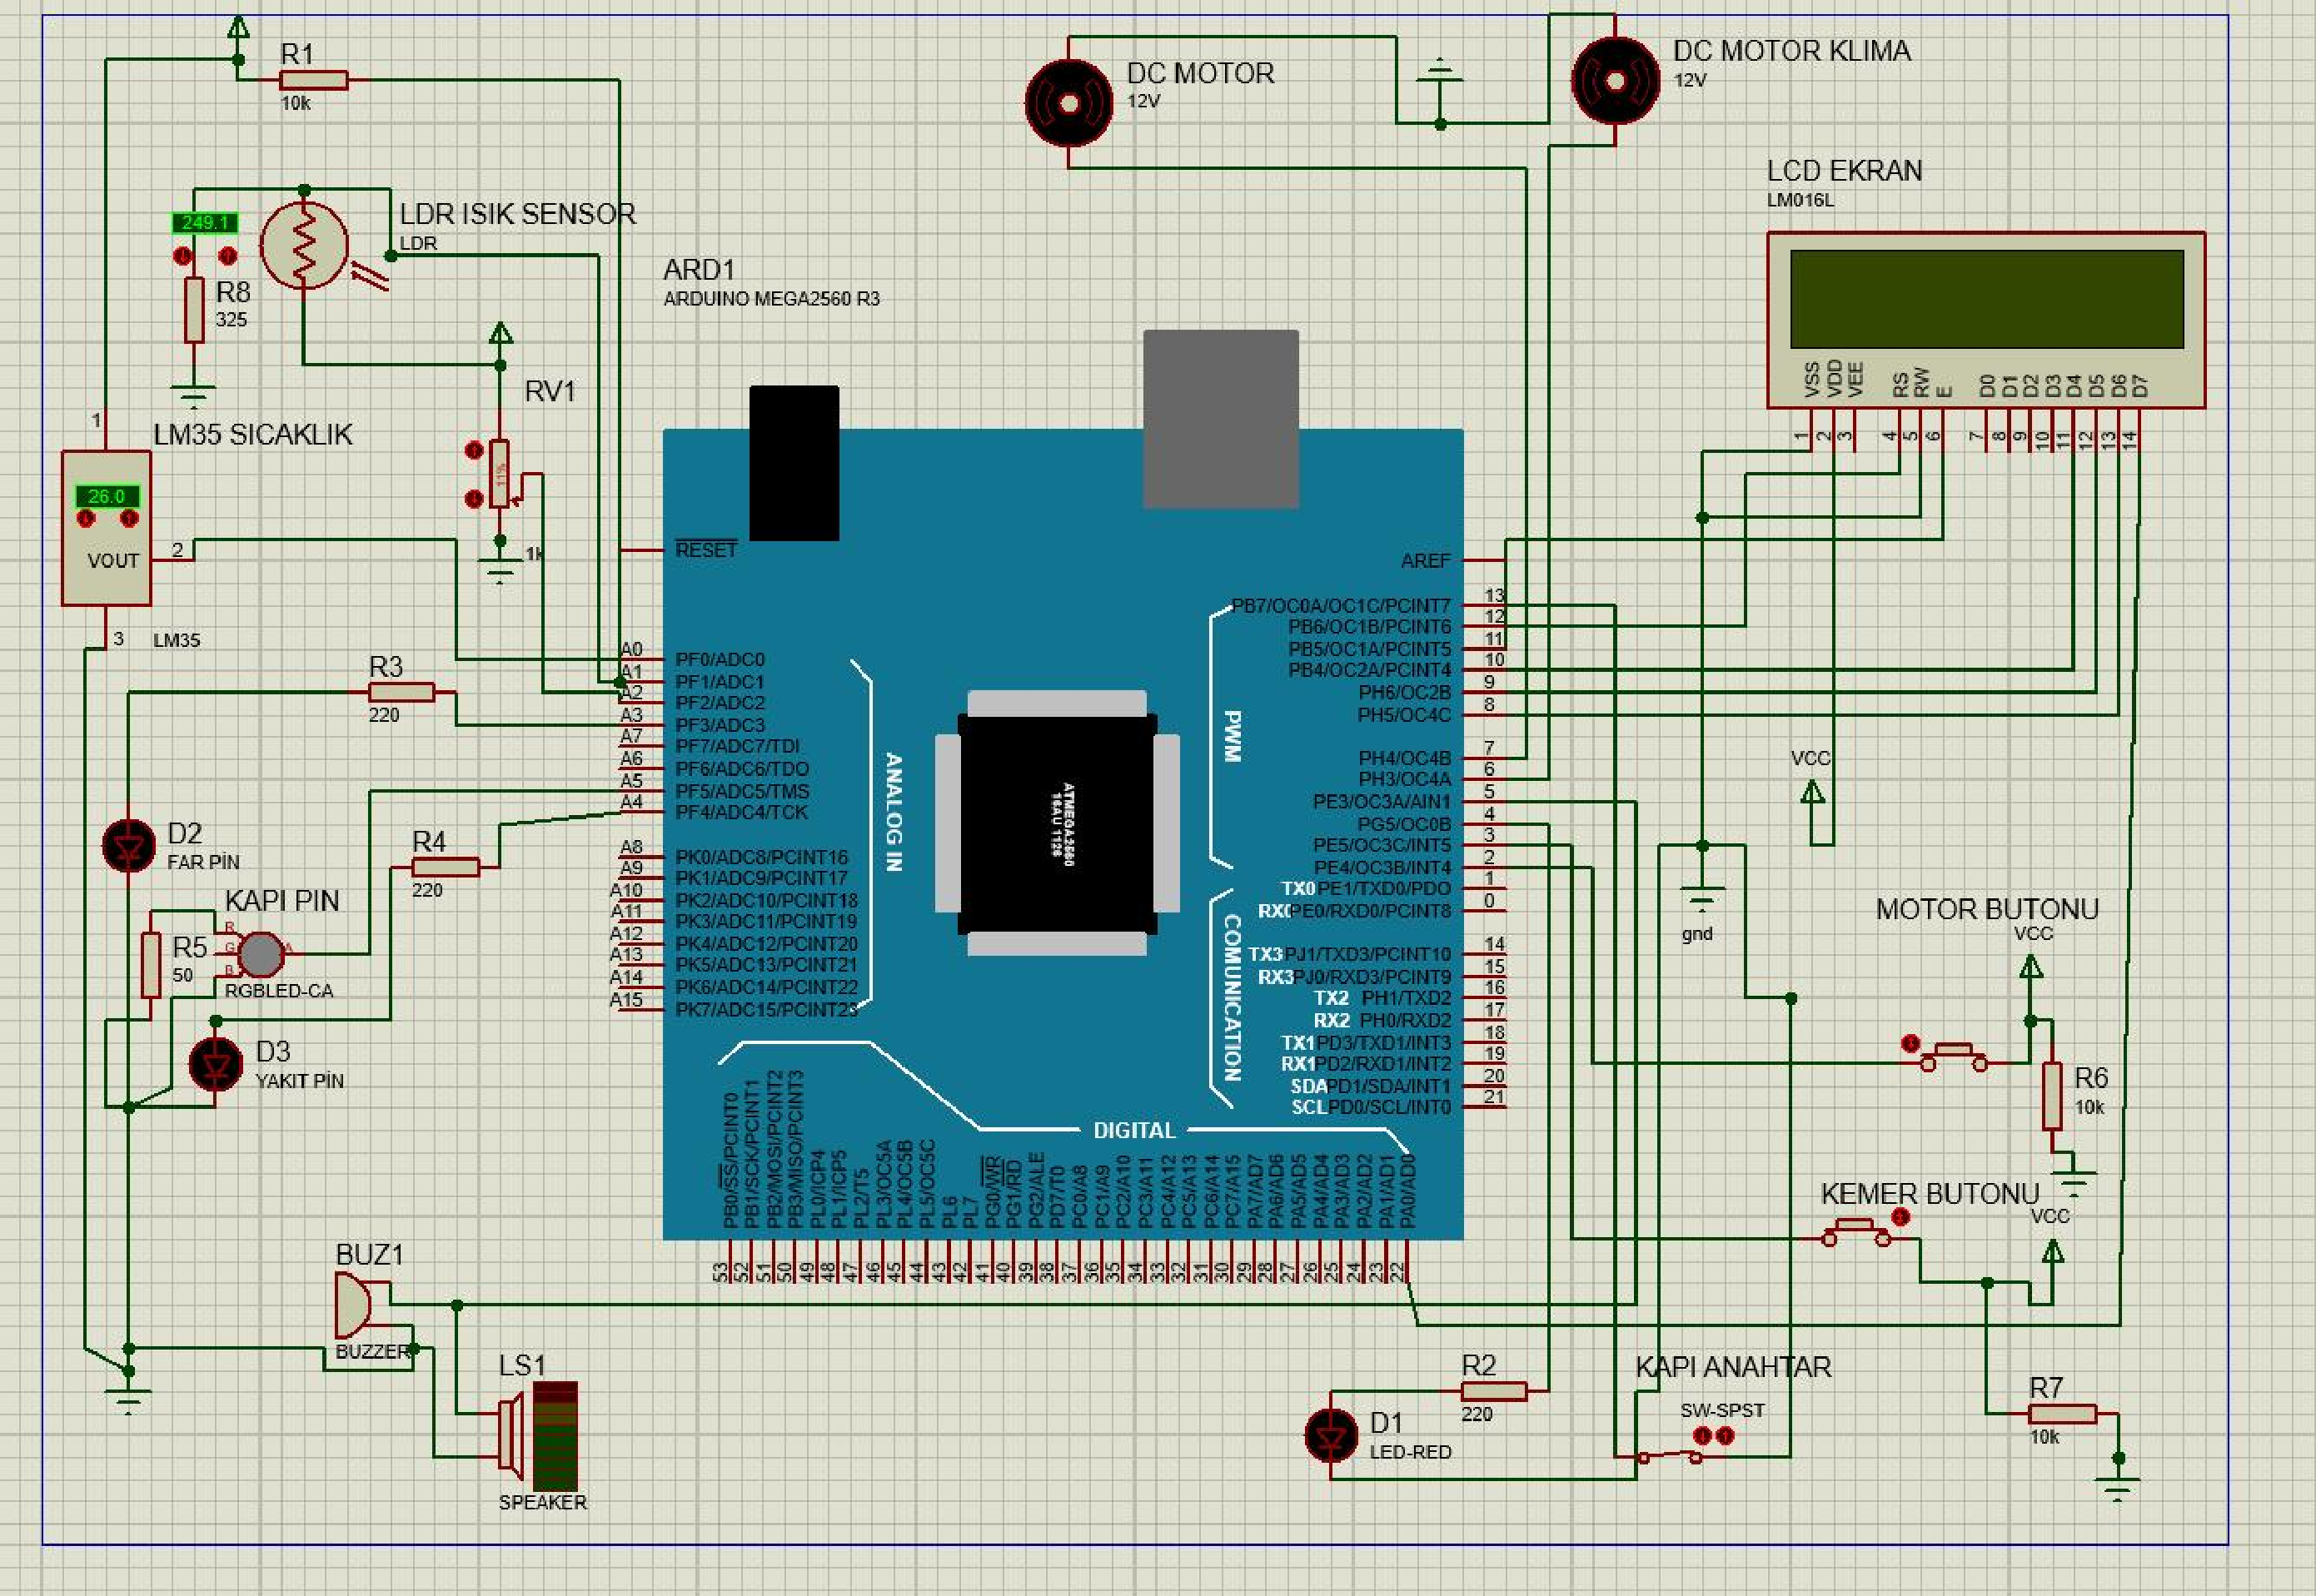
\includegraphics[width=0.47\textwidth]{simulasyon_gorselleri.pdf}
\caption{Proteus simülasyon devresi}
\end{figure}

\subsection{Donanım Bileşenleri}
\begin{itemize}
    \item \textbf{LM35 Sıcaklık Sensörü:} Ortam sıcaklığı 25°C üzerine çıktığında klima motorunu devreye sokmak için kullanılmıştır.
    \item \textbf{LDR (Işık Sensörü):} Ortamın aydınlık/karanlık olma durumuna göre far LED’ini kontrol eder.
    \item \textbf{Potansiyometre:} Analog yakıt seviyesi simülasyonu sağlar. Kritik seviyeye inildiğinde motoru durdurur.
    \item \textbf{Butonlar:} Kapı anahtarı, emniyet kemeri ve motor başlatma düğmeleri olarak kullanılır.
    \item \textbf{RGB LED ve Buzzer:} Uyarı durumlarında sesli ve görsel bildirim sağlar.
    \item \textbf{LCD Ekran:} Tüm sistem verileri kullanıcıya gösterilir.
\end{itemize}

\subsection{Yazılım Yapısı}


\section{Pseudocode}

\begin{verbatim}
BAŞLA

EĞER kapı açıksa
    Motor çalışmasın
    Uyarı mesajı ver

EĞER kemer takılı değilse
    Motor çalışmasın
    Buzzer öt

EĞER motor butonuna basılmışsa VE
     kapı kapalıysa VE kemer takılıysa
    Motor çalışsın

SICAKLIK ölç
EĞER > 25°C ise klima çalışsın

IŞIK ölç
EĞER LDR < 250 ise farlar açılsın
DEĞİLSE farlar kapansın (tek mesaj)

YAKIT ölç
EĞER < 5% ise LED yanıp sönsün
EĞER <= 0% ise motor kilitlensin

SON
\end{verbatim}

\section{Deneysel Sonuçlar}
Proteus 8 Professional ortamında oluşturulan devre tasarımında, tüm sensörler ve çıkış elemanları (LED, Buzzer, DC motor, LCD ekran) başarıyla entegre edilmiş ve sistemin farklı senaryolara verdiği tepkiler detaylı bir şekilde gözlemlenmiştir. Simülasyon süreci sırasında elde edilen başlıca bulgular şunlardır:

\begin{itemize}
    \item Emniyet kemeri takılı değilken motorun çalışması engellenmiş ve kullanıcıya LCD ekran ve buzzer aracılığıyla uyarı verilmiştir.
    \item Kapı açıkken sistem, motor çalıştırma butonuna basılsa bile motoru devreye almamış, güvenlik önceliğini korumuştur.
    \item Ortam ışığı LDR sensör tarafından algılanarak, 250 değerinin altına düşmesi durumunda far LED’i otomatik olarak aktif hâle getirilmiştir.
    \item Sıcaklık değeri 25°C eşiğini geçtiğinde klima motoru rölesi tetiklenmiş ve bu durum LCD ekranda kullanıcıya bildirilmiştir.
    \item Potansiyometre yardımıyla düşük yakıt seviyesi simüle edilmiş; yakıt oranı yüzde 5'in altına düştüğünde sarı LED yanıp sönmeye başlamış ve yüzde 0 seviyesinde motor güvenlik amaçlı durdurulmuştur.
\end{itemize}

Bununla birlikte, simülasyon sürecinde bazı zorluklar da yaşanmıştır. Özellikle Proteus ortamında buzzer gibi sesli uyarı bileşenlerini doğru şekilde simüle etmek beklenenden daha karmaşık olmuştur. Basit tone() ve noTone() komutları fiziksel devrede sorunsuz çalışırken, Proteus üzerinde doğrudan ses üretebilmek için ek olarak bir speaker (hoparlör) bileşeni kullanılması gerekmiştir. Proteus’ta Arduino'ya doğrudan buzzer bağlandığında sesin düzgün şekilde üretilemediği, bu nedenle devreye bir speaker entegre edilerek ses dalgalarının simülasyon ortamında algılanabilir hale getirildiği gözlemlenmiştir. Ancak buna rağmen, sesin gerçek dünyadaki kadar net ve sürekli olmadığı da deneyimlenmiştir.



Bu durumlar, simülasyonun gerçeği yalnızca sınırlı bir şekilde temsil ettiğini ve nihai doğrulamanın fiziksel devre üzerinde yapılmasının zorunlu olduğunu göstermektedir. 

Ayrıca gerçek zamanlı çalışan gömülü sistemlerde, donanım bağımlı işlemlerin yönetimi için daha optimize ve düşük seviye dillerin (C, C++) tercih edilmesi gerektiği bir kez daha anlaşılmıştır. Arduino IDE üzerinde yazılan kodlar, derleyici tarafından optimize edilse de, çok hassas zamanlamalara sahip sistemlerde assembly veya saf C dilinde geliştirme yapılması, sistemin yanıt süresi ve deterministik çalışması açısından kritik önem taşımaktadır.

Sonuç olarak, Proteus gibi simülasyon araçları, sistem geliştirme sürecinde erken aşamalarda büyük fayda sağlasa da, gerçek donanım testleri yapılmadan tam doğrulama yapılamaz. Bu nedenle geliştirilen sistem, ilerleyen çalışmalarda doğrudan fiziksel prototipler üzerinde de test edilerek optimize edilecektir.
\end{itemize}


\begin{figure}[H]
\centering
\includegraphics[width=0.47\textwidth]{b.png}
\caption{Proteus simülasyon devresi}
\end{figure}

\begin{figure}[H]
\centering
\includegraphics[width=0.37\textwidth]{d.png}
\caption{Proteus simülasyon devresi}
\end{figure}



\begin{figure}[H]
\centering
\includegraphics[width=0.37\textwidth]{c.png}
\caption{Proteus simülasyon devresi}
\end{figure}




\section{Sonuç}
Bu proje kapsamında geliştirilen araç içi güvenlik ve kontrol sistemi, temel gömülü sistem prensipleri kullanılarak oldukça verimli bir şekilde çalıştırılmıştır. Sistem, yalnızca simülasyon ortamında doğrulanmakla kalmamış, aynı zamanda uygun kablolama, sağlam montaj teknikleri ve sensör yerleşimi ile gerçek araçlara entegre edilebilir bir prototip niteliği kazanmıştır. Motor durdurma, ışık kontrolü, sıcaklık tabanlı klima tetiklemesi ve yakıt seviyesi yönetimi gibi işlevlerin entegre çalışması, modern akıllı araç teknolojilerinde kullanılan sistemlerin küçük ölçekli bir yansıması olmuştur.

Günümüz otomotiv sektöründe bu tür güvenlik ve kontrol sistemleri, Advanced Driver Assistance Systems (ADAS) çatısı altında çok daha karmaşık biçimde gerçekleştirilmektedir. Otomatik fren sistemleri, şerit takip asistanları, adaptif farlar ve kablosuz teşhis modülleri gibi bileşenler, CAN-Bus ve LIN protokolleri üzerinden merkezi bir ağ ile birbirine bağlanmakta ve gerçek zamanlı veri akışı sağlamaktadır. Bu çalışmada gerçekleştirilen küçük ölçekli model, bu gelişmiş sistemlerin temel prensiplerini somut bir biçimde ortaya koyarak hem akademik hem de uygulamalı bir örnek oluşturmuştur.

Sistem tasarımı sırasında yalnızca elektronik ve yazılım bilgisi değil, aynı zamanda mekanik mühendisliği prensipleri de göz önüne alınmalıdır. Gerçek bir araç ortamında, sensörlerin montajı, titreşim ve sıcaklık dayanımı, kablolama güvenliği ve elektromanyetik etkileşim gibi faktörler ciddi mühendislik problemleri doğurabilir. Bu nedenle böyle bir sistemin gerçek araçlara entegrasyonu, bilgisayar mühendisliği, elektrik-elektronik mühendisliği ve makine mühendisliği disiplinlerinden uzmanların ortak çalışmasını gerektirir. Ayrıca, sistemin uzun vadeli güvenilirliği için hata toleranslı yazılım geliştirme, enerji yönetimi ve güvenlik protokollerinin de dahil edilmesi önem arz etmektedir.

İlerleyen aşamalarda, sistemin Bluetooth üzerinden mobil cihazlarla kontrol edilebilir hâle getirilmesi, CAN-Bus uyumlu bir ağ mimarisiyle genişletilmesi ve ESP32 gibi daha güçlü Wi-Fi/Bluetooth destekli mikrodenetleyicilerle yeniden tasarlanması planlanabilir. Böylelikle araç içi veri paylaşımı ve uzaktan kontrol imkanları artırılarak, sistemin akıllı araç konseptine daha da yaklaşması sağlanabilecektir. Ayrıca yapay zekâ destekli karar sistemleriyle far kontrolü, motor güvenlik önlemleri ve yakıt tüketim optimizasyonu gibi özellikler de gelecekteki geliştirmelere entegre edilebilir.


\begin{figure}[H]
\centering
\includegraphics[width=0.57\textwidth]{Ekran görüntüsü 2025-04-27 134852.png}
\caption{Proteus ve Arduino IDE ortamımız}
\end{figure}



\begin{figure}[H]
\centering
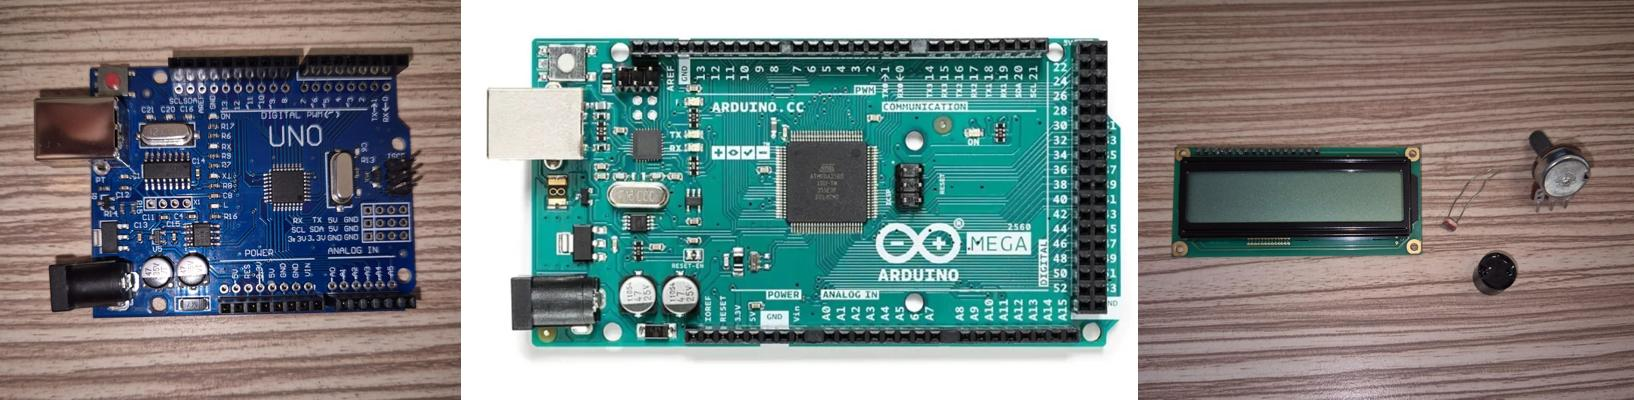
\includegraphics[width=1.0\textwidth, height=8cm]{kullanicilan_bilesenler_collage.jpg}
\caption{Gerçek kartlarımız ve sensörlerimiz,Sağdan sola Arduino UNO,Arduino MEGA ve sensörler}
\end{figure}



\section*{Kaynaklar}
\begin{itemize}
      \item Arduino Mega 2560 Datasheet, Arduino.cc
      \item LM35 Sensör Datasheet, Texas Instruments
      \item Proteus Design Suite Kullanım Kılavuzu, Labcenter
      \item C Programming for Arduino, Packt Publishing
      \item https://maker.robotistan.com/arduino-yazilim-kurulum/
      \item https://www.overleaf.com/
\end{itemize}



\end{document}
